\documentclass{scrartcl}

\usepackage[utf8]{inputenc}
\usepackage{amsmath}
\usepackage{amsthm}
\usepackage{amssymb}
\usepackage{geometry}
\usepackage{mathtools}
\usepackage{cancel}
\usepackage{xfrac}
\usepackage{siunitx}                                % for scientific notation \num{}
\usepackage{authblk}                                % for authors
\usepackage{tikz}                                   % for circled {}
\usepackage{systeme}                                % for system of equations bracket
\usepackage{verbatim}                               % for comment
\usepackage{xfp}                                    % for floating point operations in macros
\usepackage{graphicx}                               % for cropping the images
\usepackage{dsfont}                                 % for doublestroke fonts
\usepackage{float}
\usepackage{hyperref}                               % hyperlink
\usepackage[english]{babel}
\usepackage[square, numbers]{natbib}
\usepackage[nottoc, notlof, notlot]{tocbibind}     % Includes "References" in the table of contents

\bibliographystyle{abbrvnat}

\hypersetup{
	colorlinks=true, 
	citecolor=blue,
}

\AtBeginDocument{\renewcommand{\bibname}{References}}

\title{Video Prediction}
\subtitle{Independent Work Report (MAE 340, Spring 2021)}
\author{Matthew Coleman}
\date{April 26, 2022}

\begin{document}

\maketitle

\vspace{8cm}
\Large
\textit{This project represents my own work, in accordance with the University regulations.} \\
\hspace*{\fill} \large /s/Matthew Coleman
\normalsize

\newpage
\tableofcontents
\newpage

\section{Introduction}
\label{sec:intro}

While humans cannot perfectly predict the future, they are indeed capable of
inferring a great deal of information about near events in the future, and this
knowledge greatly aids them in planning out their actions, such as which
movements to take to reach a goal. This ability to forecast the future is a
direct result of an understanding of causality that is learned through
observation and interaction \cite{human_learning_sequences}.

A great amount of human predictions are erroneous in major respects, but even
the humans least adept at inferring far-off outcomes and consequences still are
masters of learning very near-term ones. For example, humans have a good sense
for where a car will move in the street, or which direction a pedestrian may
continue walking. Even a young child can predict where to toss a football to a
moving receiver, and even this small knowledge reveals an infinite wisdom
compared to the most advanced video prediction methods.

The task of video prediction is comprised of several open challenges in
computer vision; it uses some of the most recent model architectures that have
been developed and it even contends directly with an impossible task
altogether, which is to predict the future. Although it is a particularly
confusing task, it also has the potential for immense impact and immediate
practical applications, such as in autonomous driving \cite{eg_self_driving},
video interpolation \cite{eg_video_interp} and most interesting in the context
of this report, robotic control systems \cite{eg_robot_control}.

This project will examine the current state-of-the-art in video prediction
machine learning models, report on several experiments carried out by
implementing and testing such a model on various existing datasets, and attempt
to make meaningful conclusions about video prediction and learning causality.

\section{The Task of Video Prediction}
\label{sec:task}

\newcommand{\Xseq}{$\boldsymbol{X} = \left( X_1 , X_2 , X_3 \cdots X_n \right)$}
\newcommand{\Yseq}{$\boldsymbol{Y} = \left( Y_1 , Y_2 , Y_3 \cdots Y_m \right)$}
\newcommand{\Yhatseq}{
	$\hat{\boldsymbol{Y}} = 
	\left( \hat{Y}_1 , \hat{Y}_2 , \hat{Y}_3 \cdots \hat{Y}_n \right)$
}

The task of video prediction is to construct an approximation for the
completion of a sequence of frames, given only the initial sequence of frames.
Formally, given an ordered set of $n$ image frames \Xseq, the task is to
predict the latter $m$ frames of the sequence \Yseq, each frame of which having
the same dimensions, for example with $c$ channels, height $h$, and width $w$.
At each inference in training, the model predictions \Yhatseq, with the same
dimensions as the inputs, are conditioned on the input sequence
$\boldsymbol{X}$, and the model weights are updated typically by the gradient
of a loss function computed between the predictions and ground truth sequence
$\boldsymbol{Y}$ directly. Critically, since there is no human intervention or
labeling required for the model to do this, and models typically are able to
learn from the implicit temporal organiziation of the video data, video
prediction is a self-supervised task \cite{video_prediction_survey}.

% A great deal of discussion in video prediction research centers around exactly
% how these predictions are computed, specifically by testing different model
% architectures, loss functions, and training approaches, however, there is also
% a good amount of disagreement on how model predictions are actually evaluated.
% For example, models trained using pixel-wise loss functions such as MSE will
% typically prefer blurrier predictions in order to capture the underlying
% stochasticity of the data, whereas GANs will prefer to produce more realistic
% data, even if the predictions are further off the mark.

\newpage
\section{Families of Prediction Models}
\label{sec:families}

Modern video prediction models tend to adopt several canonical architectures,
which are normally simple and easily generalizable for specific tasks, such
that they can be used as building blocks or blueprints within larger
architectures. Understanding what each architecture seeks to do on a high level
is imperative to understanding what kind of output one should expect from the
model, since they are each very unique, and research implementations make use
of them in different ways.

For example, RNNs and generative networks are each successful and well-tested
paradigms used in many other machine learning domains outside of computer
vision, but they are especially utilized within video prediction because of
their key properties and strengths, particularly of RNNs to work on
time-sequential data and of generative networks to ``imagine'' new data within
a distribution. These paradigms are used extensively in Convolutional LSTM,
FutureGAN \cite{futuregan}, and SAVP models \cite{savp}, as well as many other
models in cutting-edge research. A short description of each family and its
relevance to video prediction is given below:

\subsection{Recurrent Neural Networks}
\label{subsec:rnn}

Formally, a Recurrent Neural Network (RNN) is the end-result of a mathematical
analysis of a nonlinear first-order non-homogeneous ordinary differential
equation describing the evolution of a state signal $s$ as a function of time,
along with an input signal $x$. The canonical statement of an RNN is given
below in the form of a discrete Delay Differential Equation (DDE)
\cite{rnn_and_lstm_fundamentals}:

\begin{equation}
	\begin{split}
		s_t & = W_s s_{t - 1} + W_r r_{t - 1} + W_x x_t + \theta_s \\
		r_t & = G ( s_t )
	\end{split}
	\label{eq:rnn_canonical}
\end{equation}

With $W_s$, $W_r$, and $W_x$ as weights which are either multiplied or
convolved with their respective signals, and $\theta_s$ as a bias term
which is typically added in element-wise fashion to $s$. This equation
also includes the read-out or output signal $r$, which is the activation
$G(z)$ of the state signal, and can be seen as the ``output'' of the network.
All together, this equation describes all of the moving parts of an RNN.

As a toy example (and ignoring some technical tricks that would be required to
make this actually happen), a network of this type could be capable of
transcribing seqeunces of a lecture by evaluating discrete audio samples
recorded from the event and outputting the spoken words in text form
\cite{rnn_and_lstm_fundamentals}. Another extremely common application of
vanilla RNNs is machine translation, in which the input sequence is text in one
language and the output is meant to be the translation of that text into
another language.

An easily understandable depiction of the RNN described in Equation
\ref{eq:rnn_canonical} can be found in Figure \ref{fig:rnn_arch}. This figure
also shows the ``unfolding'' or ``unrolling'' of the model, which is just a way
of seeing each time-step of the state signal $s_t$, input signal
$x_t$, and ouput signal $r_t$ (here replaced by $\hat{y}_t$,
denoting the network inferences) as they are produced over time.

\begin{figure}[H]
	\begin{center}
		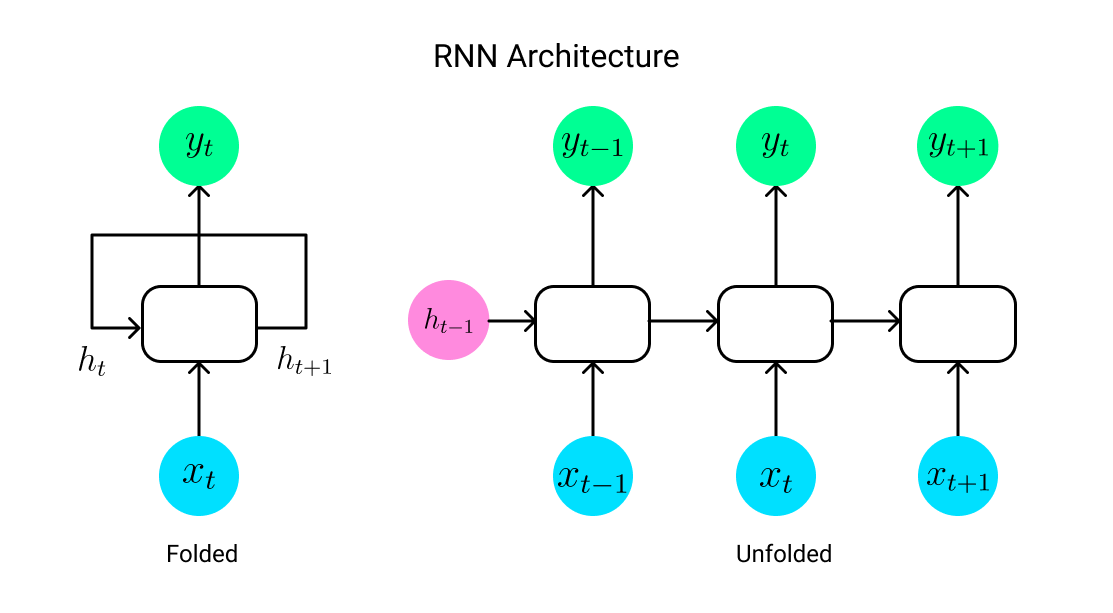
\includegraphics[width=1\textwidth]{figures/rnn_arch.png}
	\end{center}
	\caption{RNN Architecture}
	\label{fig:rnn_arch}
\end{figure}

RNNs are generally trained using a techinque called Backpropagation Through
Time (BPTT), in which the gradient of a loss function taken at a certain
instance in time is used to update the model parameters recursively through the
history of the model, using the chain rule. In this way, RNN models trained
over long sequences have their parameters updated by the product of many
Jacobian matrices, which, just like a product of many real numbers, can vanish
or explode very easily \cite{rnn_training_challenges}. For this reason, along
with several others having to do with the long-term stability of RNNs, the Long
Short-Term Memory (LSTM) cell was developed with nonlinear, data-dependent
controls in the form of several ``gates'' that control input to and output from 
the cell's state \cite{rnn_and_lstm_fundamentals}.

\subsection{Long Short-Term Memory (LSTM) Cell}
\label{subsec:lstm}

The changes described in the following section take the form of a modified
system of equations \cite{rnn_review}: 

\newcommand{\csquig}{\tilde{c}}

\begin{equation}
	\begin{split}
		f_t           & = \sigma ( W_{fh} h_{t - 1} + W_{fx} x_t + b_f ) \\
		i_t           & = \sigma ( W_{ih} h_{t - 1} + W_{ix} x_t + b_i ) \\
		\csquig_t     & = \tanh ( W_{\csquig h} h_{t - 1} + W_{\csquig x} x_t + b_{\csquig} ) \\
		o_t           & = \sigma ( W_{oh} h_{t - 1} + W_{ox} x_t + b_o ) \\
		c_t           & = f_t \circ c_{t - 1} + i_t \circ \tilde{c}_t \\
		h_t           & = o_t \circ \tanh ( c_t )
	\end{split}
	\label{eq:lstm_canonical}
\end{equation}

The key differences in the LSTM are the four gates denoted by $f$, $i$,
$\tilde{c}$, and $o$. Other than these, the cell state $c$ and output $h$ are
analogous to the original RNN definition. Now, the input and output gates are
able to ``learn'' how to add information to the cell state or take information
for inferences, and the forget gate is able to remove information from the cell
state entirely. To see how this is done, recall that the sigmoid funtion
$\sigma (z)$ has an output range of $(0, 1)$, meaning that element-wise
multiplication by embeddings activated by sigmoid can minimize and essentially
nullify the cell state. In the input gate, this same technique is applied for
$i$ onto $\tilde{c}$, and in the output gate it is applied by $o$ onto $c$,
meaning that $i$ decides what from $h_{t - 1}$ is allowed into the cell state
and $o$ decides what from $c_{t - 1}$ is allowed out of the cell state into the
inference. A diagram of these connections is shown in Figure
\ref{fig:lstmcell_arch}.

\begin{figure}[H]
	\begin{center}
		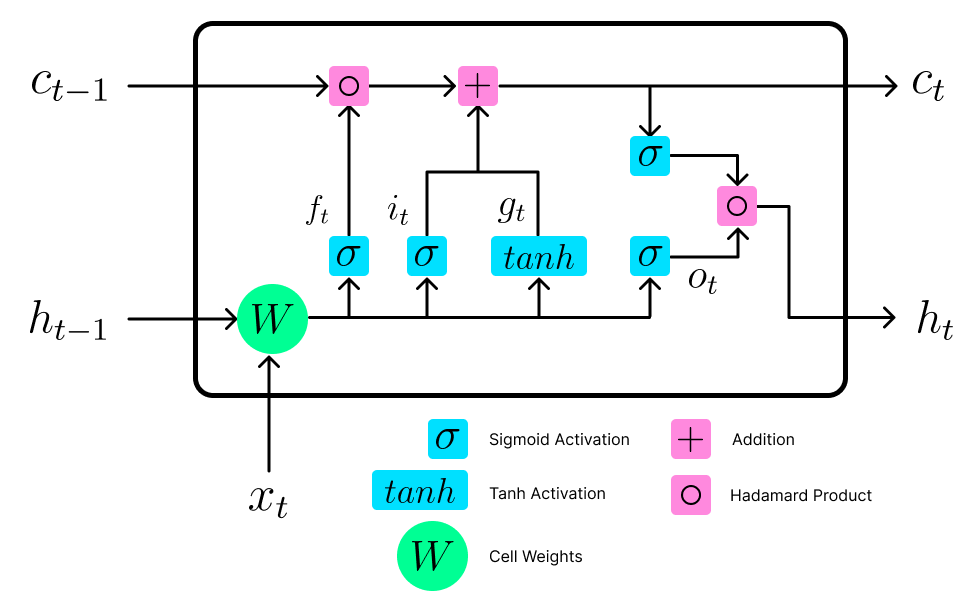
\includegraphics[width=1\textwidth]{figures/lstmcell_arch.png}
	\end{center}
	\caption{LSTM Cell Architecture}
	\label{fig:lstmcell_arch}
\end{figure}

In this way, LSTM cells are capable of mitigating some of the drawbacks of RNNs
such as vanishing and exploding gradients, and they are capable of learning how
to make good inferences for very different sequences. In other words, they are
better able to approximate both $y_{t_1}$ and $y_{t_2 \gg t_1}$ using the same
parameters.

Now that some of the general architectures and methodologies are laid out,
however, the question still remains of how these models actually predict the
continuation $\boldsymbol{Y}$ of a sequence of frames $\boldsymbol{X}$ with any
sort of accuracy. In order to do this, one final methodology must be examined,
namely Sequence to Sequence (Seq2Seq) learning, which will lead to the final
implementation of a Convolutional LSTM used for experimentation in this
project.

\subsection{Sequence To Sequence Learning}
\label{subsec:seq2seq}

Seq2Seq learning is only a slight modification to the original usage of RNNs,
but they represent an elegant solution to a classical shortcoming of most Deep
Neural Networks (DNNs), which is that, despite their flexibility, they can only
be applied to problems in which inputs and outputs can fit into fixed,
discretized, vectors, and therefore must be of a certain length or size.
Seq2Seq learning solves this problem for video prediction as well as many other
tasks by using 2 LSTMs: an encoder to read the sequence and learn to create an
embedding vector, and a decoder, which is passed the embedding vector and
learns to generate the predicted sequence \cite{seq2seq_original}. A diagram of
this procedure is shown in Figure \ref{fig:seq2seq_arch}.

\begin{figure}[H]
	\begin{center}
		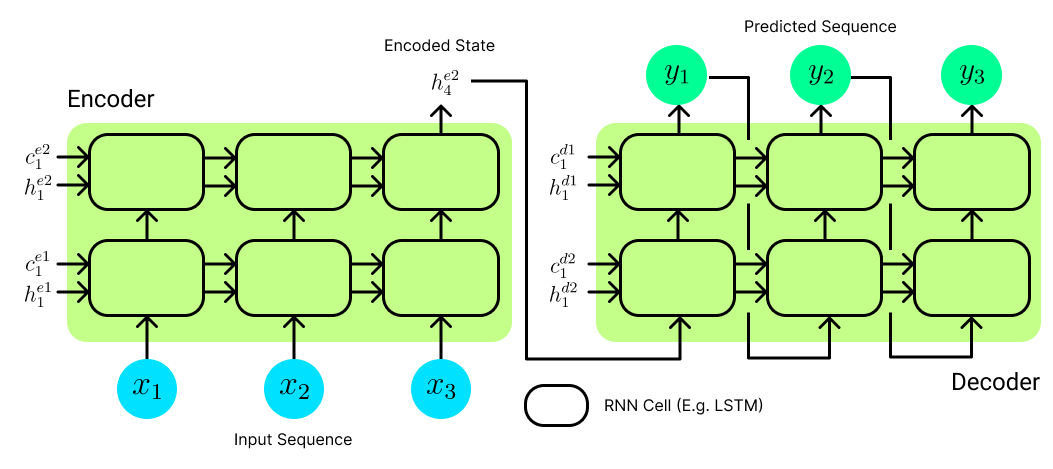
\includegraphics[width=1\textwidth]{figures/seq2seq_arch.png}
	\end{center}
	\caption{Seq2Seq Architecture}
	\label{fig:seq2seq_arch}
\end{figure}

The diagram shows how the input sequence $x$ is fed into the encoder LSTM for 3
steps (in practice this can be any length), how the encoder generates an
embedding vector $h_4$ which is passed to the decoder as an input, and how the
decoder generates the predicted sequence by passing the predicted output
$\hat{y}_{t}$ back into itself at the next time step as an input, continuing until
all predicted frames are generated.

This diagram also shows two layered LSTM cells, which is another key
modification used in this project's implementation. Note that each layer has
it's own states $h$ and $c$, and at each time step, the cells pass their $h$
embedding up to the next cell as an input. Deep, multilayered LSTMs have been
shown to significantly outperform shallow LSTMs for language translation
\cite{seq2seq_original}, however, this project will also analyze the effect of
depth on LSTM inferences for video prediction. 

In sum, these are the main methods used in this report's implementation of an
LSTM model for video prediction, which can be found at this
\href{https://github.com/msc5/junior-iw}{GitHub repository}.

% \subsection{Generative Models}
% \label{subsec:generative}
%
% \begin{figure}[H]
% 	\begin{center}
% 		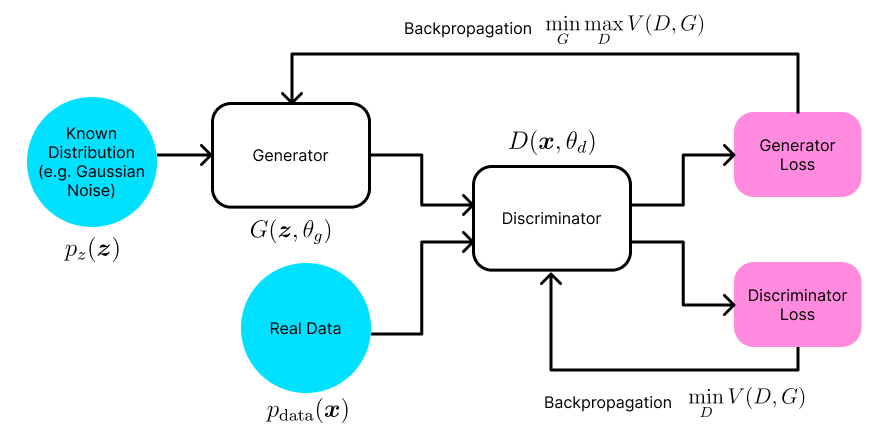
\includegraphics[width=1\textwidth]{figures/gan_arch.png}
% 	\end{center}
% 	\caption{General GAN Architecture}
% 	\label{fig:gan_arch}
% \end{figure}
%
% Generative neural networks (for example, GANs) consist of mostly the same
% architecture as discriminative neural nets, such as the ones which are
% classically used for image classification. While discriminative nets seek to
% learn the conditional probability $p(y \mid x)$ of an input $x$ belonging to a
% particular class $y$, generative nets seek to learn the conditional probability
% distribution $p(x \mid y)$ of an input data given the output, allowing them to
% make inferences in the form of ``imagined'' data that might belong to the same
% distribution as $x$ \cite{gan_original}. In short, discriminative models would
% look at many Van Gogh paintings and fakes in order to learn to differentiate
% between them, and generative models would look at many Van Gogh paintings in
% order to learn how to paint like Van Gogh.
%
% In practice, this is done by passing a low-dimensional embedding vector from a
% known latent distribution (such as the kind that may come as an activation from
% a discriminative net) through a typical network in reverse, generating an
% upscaled output in the same shape as the targeted learning data.

% \section{Video Prediction Models}
% \label{sec:families}

% \subsection{Convolutional LSTM}
% \label{subsec:conv_lstm}
%
% \subsection{FutureGAN}
% \label{subsec:futuregan}
%
% \begin{figure}[H]
% 	\begin{center}
% 		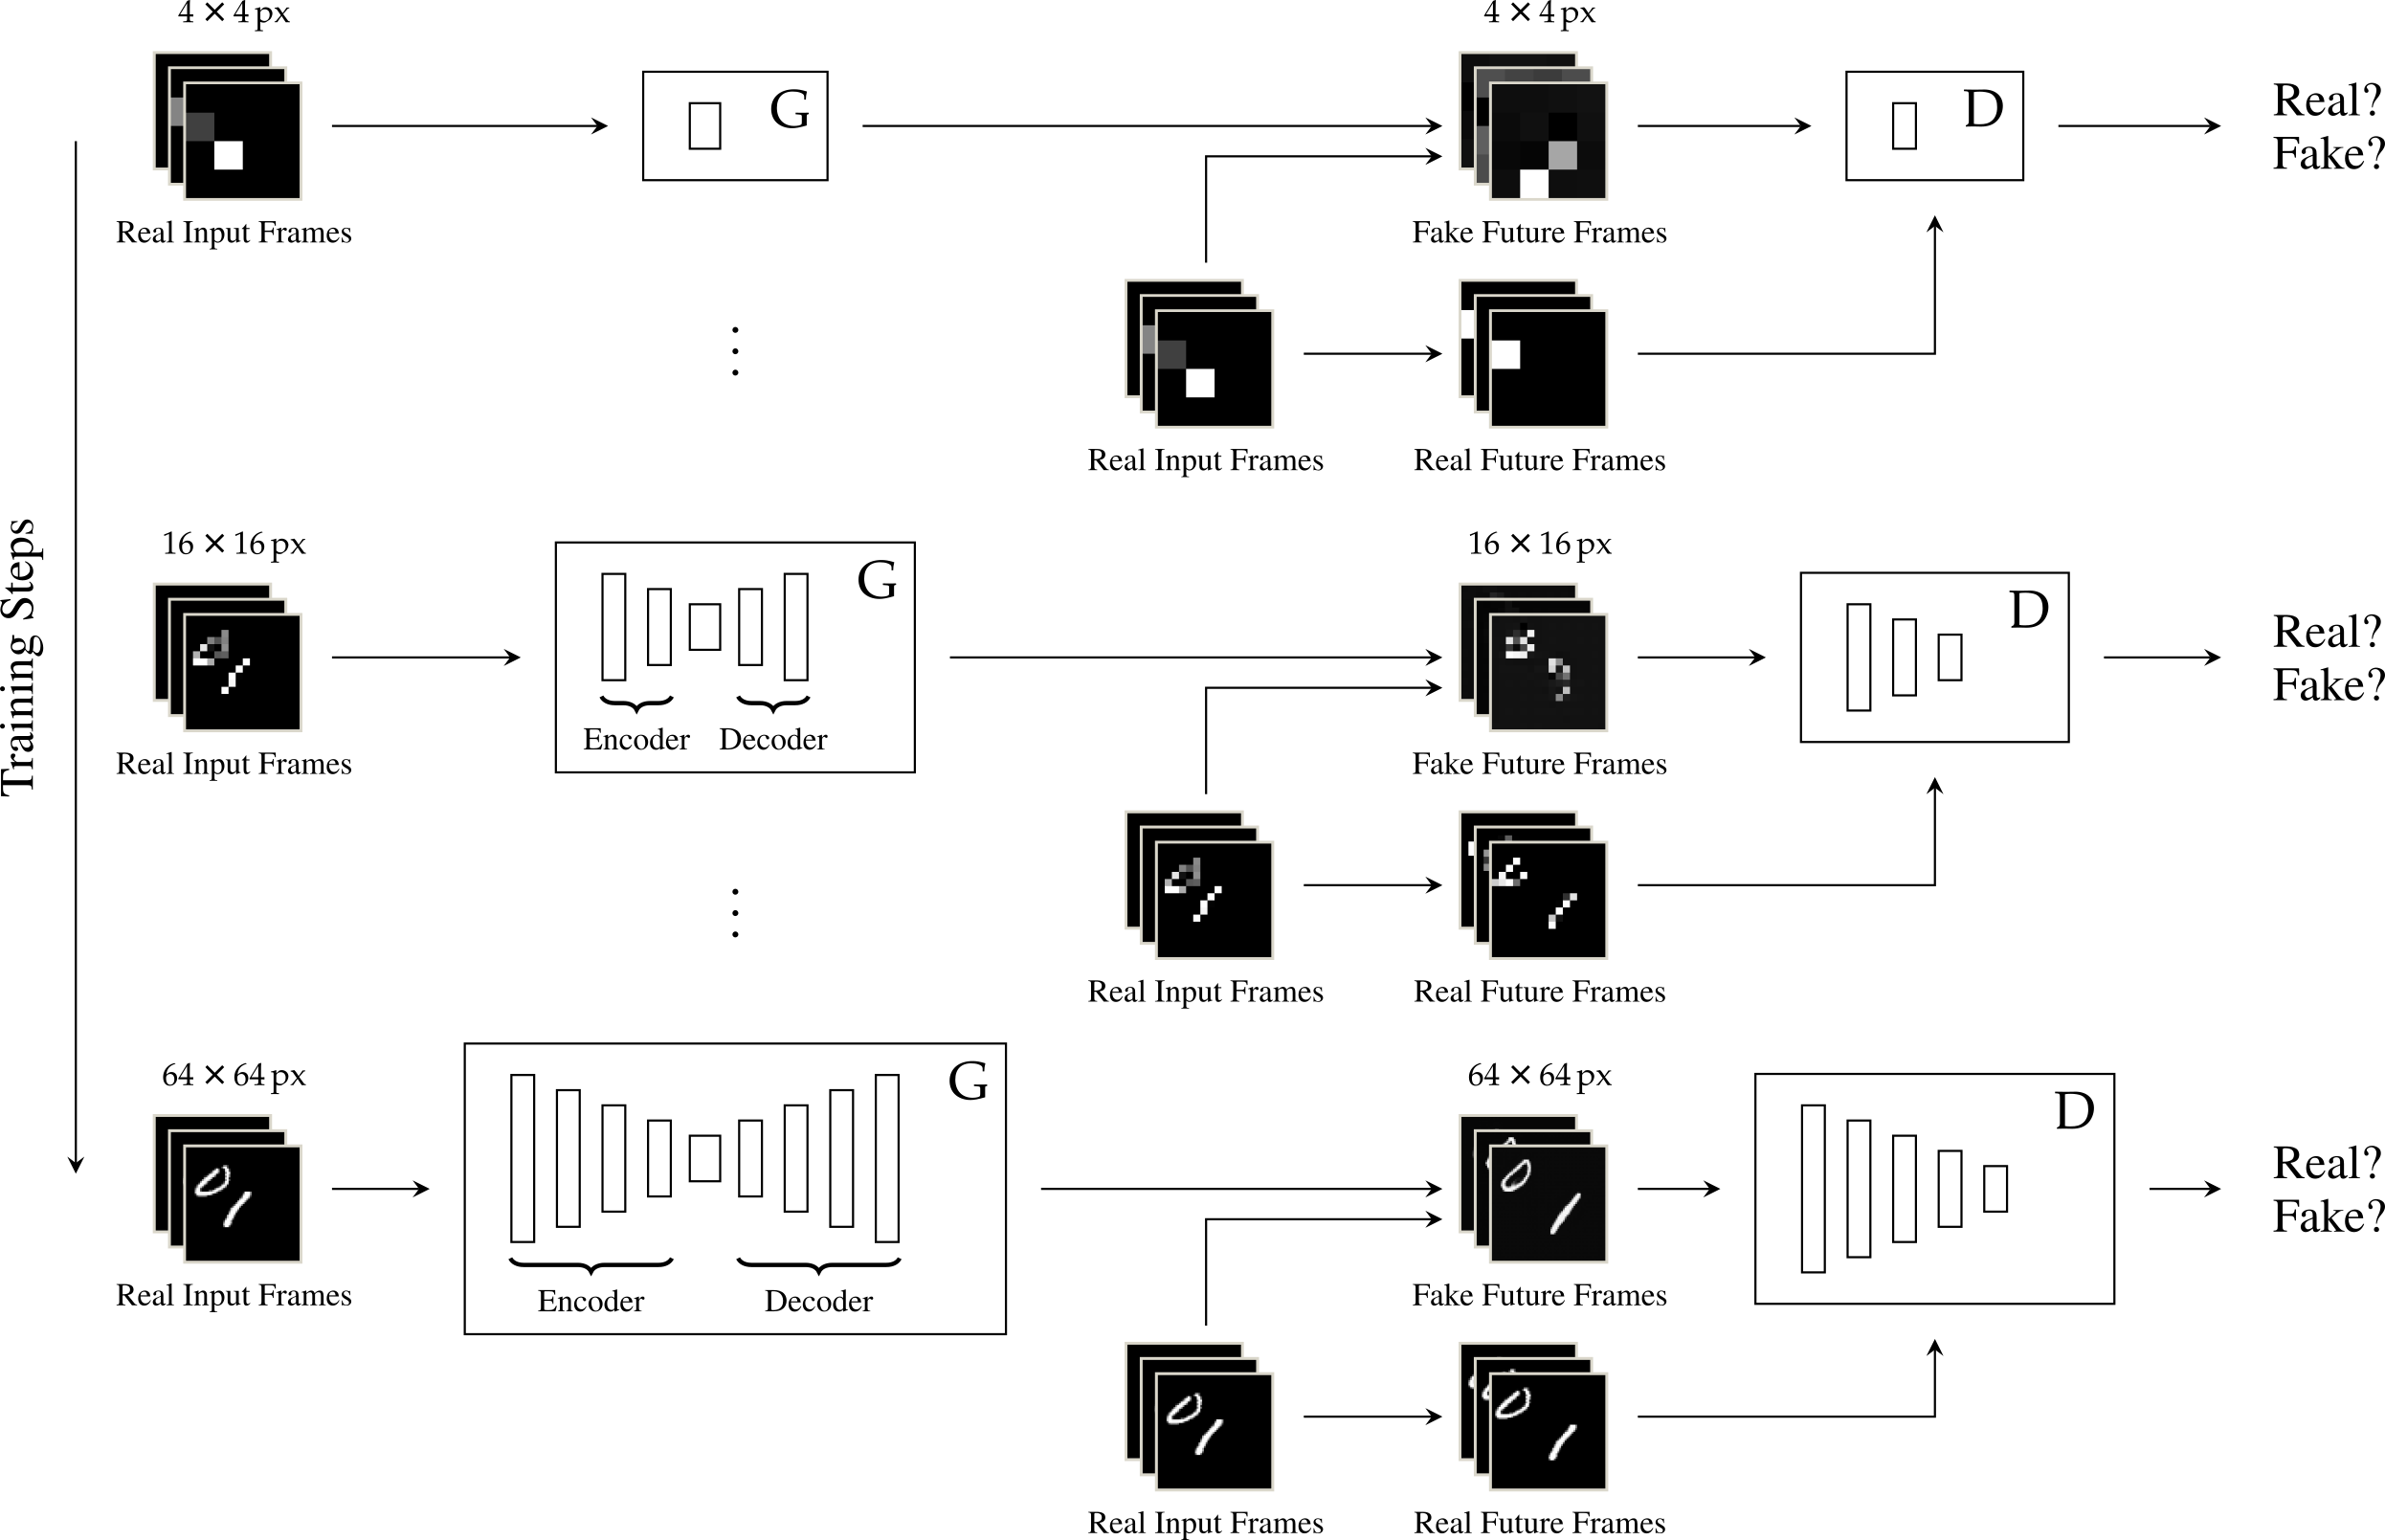
\includegraphics[width=1\textwidth]{figures/futuregan_arch.png}
% 	\end{center}
% 	\caption{FutureGAN Architecture}
% 	\label{fig:futuregan_arch}
% \end{figure}
%
% \subsection{SAVP}
% \label{subsec:savp}

\newpage
\section{Datasets}
\label{sec:datasets}

\subsection{MovingMNIST}
\label{subsec:mmnist}

\subsection{KTH}
\label{subsec:kth}

\subsection{BAIR}
\label{subsec:bair}

\newpage
\section{Experiments}
\label{sec:experiments}

% \begin{table}
% 	\caption{Summary of Main ConvLSTM Results}
% 	\label{tab:results_summary}
% 	\begin{center}
% 		\begin{tabular}{ l l l l }
% 			\textbf{Dataset} & \textbf{Number of layers} & \textbf{Number of Parameters} & \textbf{Test MSE Loss} \\
% 			MovingMNIST & \\
% 			KTH & \\
% 			BAIR
% 		\end{tabular}
% 	\end{center}
% \end{table}

The main experimental procedure carried out in this report is the training and
testing of the re-implemented Convolutional LSTM model on the MovingMNIST, KTH,
and BAIR datasets, however, in order to more gain a more robust understanding
of LSTM features and limitations, as well as to debug the training mechanisms
in a much simpler setting, it was useful to first test a Linear LSTM model on
one-dimensional sequential data before moving fully to video prediction.

This Linear LSTM was implemented with nearly the same exact architecture as the
Convolutional LSTM, however with Linear layers in place of convolutions, and as
a result, a 2D convolution layer as the final step as opposed to 3D.

% Insert Linear LSTM specifics

\subsection{Sequence Prediction}
\label{subsec:experiment_sp}

Two generated datasets of one-dimensional sequences were implemented, one which
was composed of sin waves with random frequency and phase offset, and another
which represented random points chosen at several steps within the sequence and
simply interpolated using a sinusoidal interpolation function. Both datasets
were normalized to the range $(0, 1)$, with 20 total data points for each
seqeuence. The model was then given the first 10 points and tasked to predict
the last 10.

\subsubsection{Generated Sinusoids}
\label{subsubsec:generated_sins}

% Figure \ref{fig:gen_sin_training} shows the model's inferences on a held-out
% set of the generated sinusoidal data as the model trains over one epoch. 

\subsection{Video Prediction}
\label{subsec:experiment_vp}

\begin{figure}[H]
	\begin{center}
		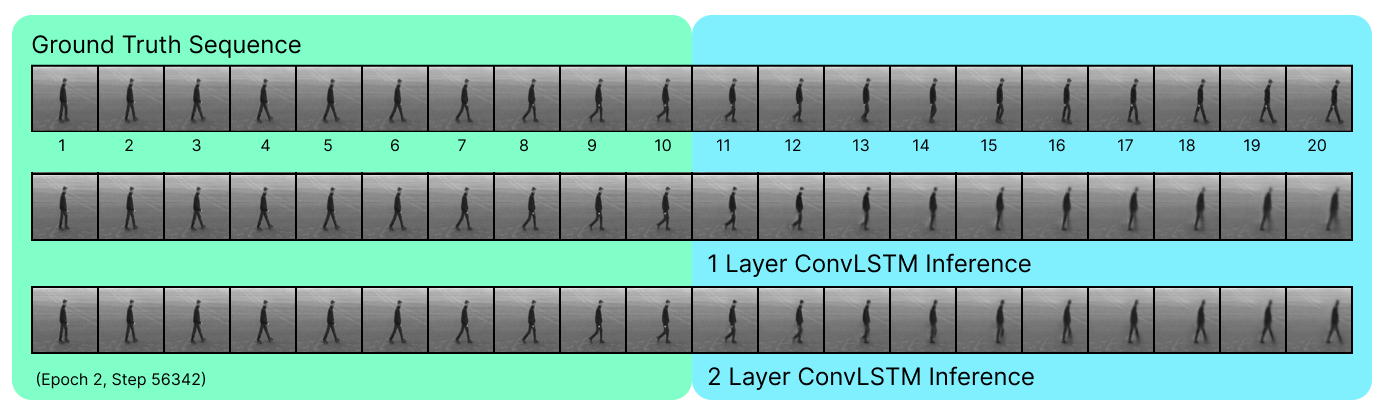
\includegraphics[width=1\textwidth]{images/kth/KTHEpoch2Step56342.png}
	\end{center}
	\caption{Convolutional LSTM Inference on KTH dataset}
	\label{img:lstm_kth_inference}
\end{figure}

\newpage
\section{Conclusion}
\label{sec:conclusion}

% ------------------------------------------------------------------------------
% References 
% ------------------------------------------------------------------------------

\newpage
\bibliography{main}
\newpage

\end{document}

